\section{Node.js}
\label{sec:node}
%% \begin{figure}
%% 	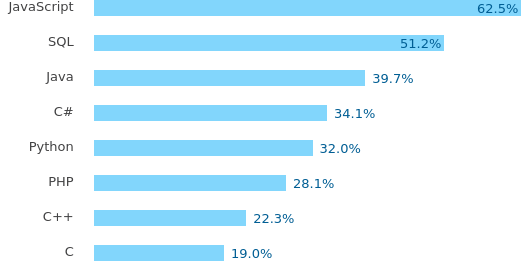
\includegraphics[width=.5\textwidth]{fig/languages}
%% 	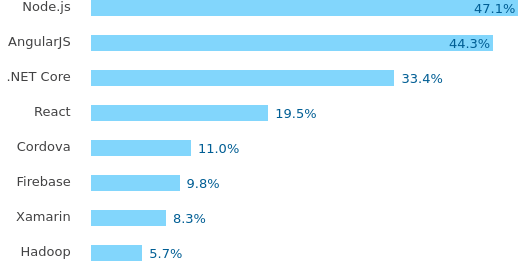
\includegraphics[width=.5\textwidth]{fig/frameworks}
%% 	\caption{Stack Overflow Developer Survey 2017, \url{https://insights.stackoverflow.com/survey/2017}. Most used programming languages (on the left) and frameworks (on the right).}
%% 	\label{fig:popularity}
%% \end{figure}
%\paragraph{JavaScript}
%According to a survey conducted among developers all over the world by the Stack Overflow website, JavaScript is currently the most popular programming language (\Cref{fig:popularity}), having been a de facto standard for client-side web development for a long time.

%JavaScript is a high-level, dynamic scripting language supporting multiple paradigms: imperative, object-oriented, event-driven and functional programming.
%Standardized as EcmaScript \cite{EcmaScript}, the language is under active development and new features are constantly added, with the latest stable version released in June 2017.

%\paragraph{Node.js}
%Node.js\footnote{\url{https://nodejs.org/}} is a JavaScript runtime environment expressly devised for running JavaScript code outside web browsers;
%since its release in 2009, its popularity has quickly increased together with JavaScript, as witnessed, for instance, by the most recent\footnote{Most popular languages and frameworks on \url{https://insights.stackoverflow.com/survey/2018}.} Stack Overflow Developer Surveys. %(\Cref{fig:popularity}).
%, thus giving developers the opportunity to use the language to write server-side code as well.

%% Node.js is based on Chrome V8, a highly optimized JavaScript engine developed for the Google Chrome web browser.
%% Furthermore, developers can count on a huge package ecosystem\footnote{\url{https://www.npmjs.com/}} with a repository of hundreds of thousand modules that can be reused.
%More recently, Node.js has become relevant for the Internet of Things as well, both because of the availability of packages for device management and its asynchronous model, which is well suited for distributed environments.
%Node-RED\footnote{\url{https://nodered.org/}} is a tool based on Node.js to support flow-based programming for the Internet of Things to connect together devices at the edge of the network.

\paragraph{Asynchronous Computation}
%The execution model of Node.js is quite different from most of other environments.
In Node.js, %%connection to databases, HTTP requests, access to the file system and every other
I/O intensive operations are by default \emph{asynchronous}: operations are only scheduled, and the program proceeds without waiting for their completion.
Computations needed to be executed after completion of I/O operations are handled with \emph{callbacks}: when an asynchronous function is invoked, a callback is passed and registered, and then invoked on the results of the operation.

The core of Node.js execution model is based on the notion of \emph{event loop}: Asynchronous requests are processed from a simple loop,
and the corresponding I/O intensive operations are scheduled for execution together with their callbacks.
The event loop is run after the whole current Node.js script is evaluated.
The idea of an event loop was popularized a long time before Node.js came in the E programming language \cite{eventloop}.

The use of asynchronous functions requires care since I/O operations requested in the same event loop are scheduled non deterministically;
if one wants to be sure that request $r_2$ is scheduled only after request $r_1$ has been completed, then
$r_2$ must be necessarily registered in the callback passed to the function call corresponding to $r_1$.

\begin{figure}
\begin{minipage}{.5\linewidth}
\begin{lstlisting}
const http = require('http');
for (let i = 1; i <= MAX; i++) {
 const req = http.request({port:'80', method:'POST'});
 req.end(String(i));
}
\end{lstlisting}
\end{minipage}
\begin{minipage}{.5\linewidth}
\begin{lstlisting}
const http = require('http');
function request(i) {
 if (i <= MAX) {
  const req = http.request({port:'80', method:'POST'});
  req.end(String(i), () => request(i+1));
 }
}
request(1);
\end{lstlisting}
\end{minipage}
\caption{Wrong (left) and correct (right) uses of the HTTP module.}
\label{lst:wrongreq}
\end{figure}
Let us consider for instance the simple example of incorrect use of the \lstinline{http.request} and \lstinline{end} asynchronous method to send HTTP request from a client, as shown in \Cref{lst:wrongreq}.
%
%\caption{Incorrect use of the asynchronous function \lstinline{request} of the \lstinline{http} module}
%\label{lst:async}
%
Such a code uses the function \lstinline{http.request} and the method \lstinline{end} to send  \lstinline{MAX} HTTP POST requests,
each one carrying as data a distinct integer (properly converted to a string)
between \lstinline{1} and \lstinline{MAX}. Since all requests are processed in the same initial event loop, they are
scheduled in a non deterministic order; as a consequence, there is no guarantee that the HTTP server will receive
the integer data in the standard order of the for loop. What is worse, the program is doomed to crash, for sufficiently high values of
\lstinline{MAX}, with a JavaScript ``heap out of memory'' fatal error, because Node.js uses an event queue to store all I/O operations
requested with asynchronous functions.

Because of non-determinism, such kinds of errors are hard to be detected with debugging or testing, while they can be caught with RV; in the example above, it suffices to monitor that the request with integer $i+1$ is processed after the invocation of the callback passed to the method \lstinline{end} of the request with integer $i$.
The reader can compare the wrong example with the correct solution on the right, where a callback is passed to \lstinline{end} as second optional argument.
%
%% \Cref{lst:async} shows the different programming patterns using synchronous and asynchronous calls in Node.js.
%% On the left, the program is blocked until the result of \lstinline{readFileSync} is returned, and then it is stored in \lstinline{data}.
%% On the right, \lstinline{fs.readFile} \emph{immediately returns} and the I/O operation is scheduled for execution together with the anonymous callback; when the result will be available, the callback will be executed receiving such result as an argument (together with an error, if any).
%% %% Node.js heavily takes advantage of the right pattern (for the sake of brevity, error handling is ignored in the example).

%% \begin{figure}[h]
%% \begin{minipage}{.5\textwidth}
%% \begin{lstlisting}
%% const fs = require('fs');
%% // the following blocks until file is read
%% const data = fs.readFileSync('/file.md');
%% // file content available
%% \end{lstlisting}
%% \end{minipage}
%% \begin{minipage}{.5\textwidth}
%% \begin{lstlisting}
%% const fs = require('fs');
%% fs.readFile('/file.md', (err, data) => {
%%   if (err) throw err;
%%   // file content available
%% });
%% \end{lstlisting}
%% \end{minipage}
%% \caption{
%%   %%Difference between synchronous and asynchronous I/O.
%%   \url{https://nodejs.org/en/docs/guides/blocking-vs-non-blocking/}}
%% \label{lst:async}
%% \end{figure}

%% As a more significant example, let us consider web requests.
%% Node.js is typically used as a server-side JavaScript environment in web development.
%% Because of this, its library offers many features that greatly simplify the task of setting up a web server.
%% For instance, it only takes a few lines of code to obtain a (very simple) HTTP server, as shown in \Cref{lst:http}.

%% \begin{figure}[h]
%% \begin{lstlisting}
%% const http = require('http');
%% const server = http.createServer((request, response) => {
%% 	request.on('data', chunk => console.log('some data received'));
%% 	request.on('end', () => response.end('ok'));
%% });
%% server.listen(80);
%% \end{lstlisting}
%% \caption{A basic web server in Node.js based on the \lstinline{http} module.}
%% \label{lst:http}
%% \end{figure}
%% The web server is created by passing a callback that will be invoked on every incoming request.
%% Such a function will receive both the request and the response object through which it can reply.

%% For each request, first a callback logging a message for every received chunk of data is registered, then a response is sent back to the client when
%% the whole request has been received. %%there is no more data.
%% Finally, the server start listening at the standard HTTP port \texttt{80}.

%% \paragraph{Event Loop}
%% The core of Node.js is the \emph{event loop}, represented in \Cref{fig:eventloop}.
%% Asynchronous requests are processed from a simple loop, and the corresponding I/O intensive operations are scheduled for execution together with their callbacks.
%% The event loop is run after the whole Node.js script is evaluated.

%% \begin{figure}[h]
%% 	\centering
%% 	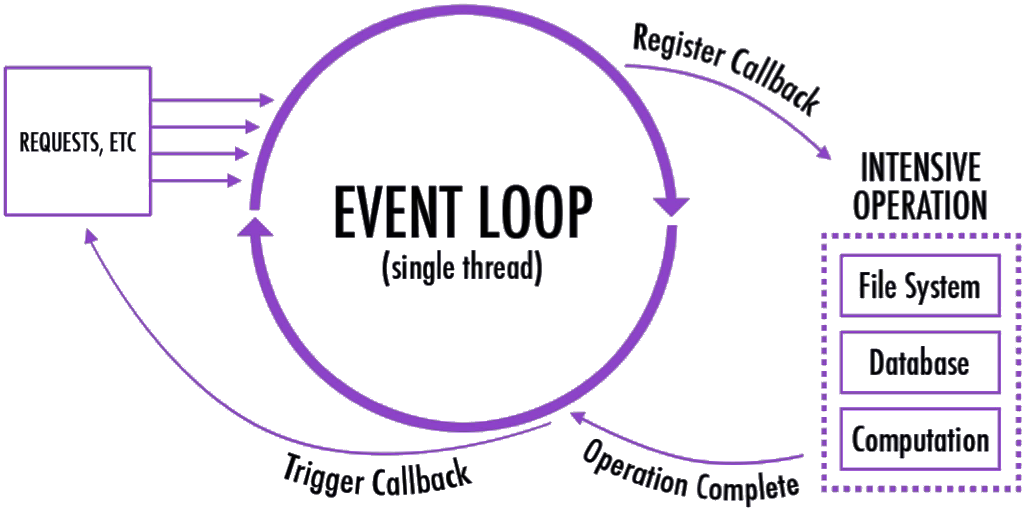
\includegraphics[width=.5\textwidth]{fig/event-loop}
%% 	\caption{Node.js execution model representation based on the event loop.}
%% 	\label{fig:eventloop}
%% \end{figure}

%% Note that callbacks themselves can make more asynchronous requests to the event loop, and those requests will receive callbacks, and so on\dots{}
%% Indeed, in real programs callbacks and I/O operations are usually nested into each other as a synchronization mechanism, making it hard to understand (and debug) the code.

%% The idea of an event loop was popularized a long time before Node.js came in the E programming language \cite{eventloop}.

%% Even if it may seem counterintuitive at first, this execution model based on asynchronous I/O and the event loop scales very well to a lot of concurrent operations, without the need for the programmer to explicitly deal with concurrency and parallelism \cite{Nodejs10,NodejsPerformance14}.
%% At the system level, different I/O operations can be executed in parallel.
